%\allowdisplaybreaks
%\section{HẰNG ĐẲNG THỨC ĐÁNG NHỚ} % Tên bài
\subsection{Tìm x}
\subsubsection{Kiến thức trọng tâm}
\begin{tomtat}
	\begin{enumerate}
		\item $\left(A+B\right)^2=A^2+2AB+B^2$;
		\item $\left(A-B\right)^2=A^2-2AB+B^2$;
		\item $A^2-B^2=\left(A-B\right) \cdot\left(A+B\right)$;
		\item $\left(A+B \right)^3=A^3+3A^2B+3AB^2+B^3$;
		\item $\left(A-B \right)^3=A^3-3A^2B+3AB^2-B^3$;
		\item $A^3+B^3=\left(A+B\right) \cdot\left(A^2-AB+B^2\right)$;
		\item $A^3-B^3=\left(A-B\right) \cdot\left(A^2+AB+B^2\right)$.
	\end{enumerate}
	$\bullet$ \textbf{\textit{Các hằng đẳng thức và kết quả mở rộng.}}
	\begin{enumerate}
		\item $A^2+B^2=\left( A+B\right) ^2-2AB$;
		\item $\left(A+B+C\right) ^2=A^2+B^2+C^2+2AB+2BC+2AC$;
		\item $\left(A-B+C\right) ^2=A^2+B^2+C^2-2AB-2BC+2AC$;
		\item $\left(A+B-C\right) ^2=A^2+B^2+C^2+2AB-2BC-2AC$;
		\item $\left(A-B-C\right) ^2=A^2+B^2+C^2-2AB+2BC-2AC$;
		\item $A^n+B^n=(A+B)(A^{n-1}+A^{n-2}\cdot B+A^{n-3}\cdot B^2+\cdots+A^2\cdot B^{n-3}+A\cdot+ B^{n-2}+B^{n-1})$.
	\end{enumerate}
\end{tomtat}
\begin{vd}%[Dự án EX-9-Đề Cương Toán 8]%[BUINHI]%[8D1H3-1]
	Tìm $x$
	\begin{multicols}{2}
		\begin{enumerate}
			\item $\left(x+7\right)^2-x\left(x-3\right)=12$;
			\item $27x^2\left(x+1\right)-\left(3x+1\right)^3=8$.
		\end{enumerate} 
	\end{multicols}
\loigiai{
		\begin{enumerate}
			\item 
			\begin{eqnarray*}
				&&x^2+14x+49-x^2+3x=12\\
				&&17x=-37\\
				&&x=-\dfrac{37}{17}.\\
				&&\text{Vậy } x=-\dfrac{37}{17}.
			\end{eqnarray*}
			\item 
			\begin{eqnarray*}
				&&27x^2\left(x+1\right)-\left(3x+1\right)^3=8\\
				&&27x^3+27x^2-\left(27x^3+27x^2+9x+1\right)=8\\
				&&-(9x+1)=8\\
				&&9x=-9\\
				&&x=-1.\\
				&&\text{Vậy } x=-1.
			\end{eqnarray*}
		\end{enumerate}
}
\end{vd}
\subsubsection{Bài tập vận dụng}
\begin{bt}%[Dự án EX-9-Đề Cương Toán 8]%[BUINHI]%[8D1H3-1]
	Tìm $x$
	\begin{enumerate}
		\begin{multicols}{2}
			\item $(x+7)^2-x\cdot (x-3)=15$;
			\item $(x-2)^2-(x+1)(x+3)=-7$;
			\item $(2x+3)^2-4x^2=10$;
			\item $(x+1)^2-(x+2)(x+3)=0$;
			\item $(x-2)^2-x(x-5)-3=0$;
			\item $9x^2-6x-3=0$;
			\item $x^3+9x^2+27x+19=0$;
			\item $x(x+5)(x-5)-(x+2)(x^2-2x+4)=3$.
		\end{multicols}
	\end{enumerate}
	\loigiai{
		\begin{enumerate}
				\item 
				\begin{eqnarray*}
					&&(x+7)^2-x\cdot (x-3)=15\\
					&&x^2+14x+49-x^2+3x=15\\
					&&17x=-34\\
					&&x=-2\\
					&&\text{Vậy }x=-2.
				\end{eqnarray*}
				\item 
				\begin{eqnarray*}
					&&(x-2)^2-(x+1)(x+3)=-7\\
					&&x^2-4x+4-x^2-4x-3=-7\\
					&&-8x=-8\\
					&&x=1.\\
					&&\text{Vậy }x=1.	
				\end{eqnarray*}	
				\item 
				\begin{eqnarray*}
					&&(2x+3)^2-4x^2=10\\
					&&4x^2+12x+9-4x^2=10\\
					&&12x=1\\
					&&x=\dfrac{1}{12}.\\
					&&\text{Vậy }x=\dfrac{1}{12}.\\
				\end{eqnarray*}
				\item 
				\begin{eqnarray*}
					&&(x+1)^2-(x+2)(x+3)=0\\
					&&x^2+2x+1-x^2-5x-6=0\\
					&&-3x=5\\
					&&x=-\dfrac{5}{3}.\\
					&&\text{Vậy }x=-\dfrac{5}{3}.
				\end{eqnarray*}
				\item 
				\begin{eqnarray*}
					&&(x-2)^2-x(x-5)-3=0\\
					&&x^2-4x+4-x^2+5x-3=0\\
					&&x=-1.\\
					&&\text{Vậy }x=-1.
				\end{eqnarray*}
				\item 
				\begin{eqnarray*}
					&&9x^2-6x-3=0\\
					&&\left[ (3x)^2-2\cdot 3x\cdot 1+1^2\right]-4=0\\
					&&(3x-1)^2-2^2=0\\
					&&(3x-1-2)\cdot(3x-1+2)=0\\
					&&(3x-3)\cdot (3x+1)=0\\
					&&3x-3=0 \text{ hoặc } 3x+1=0\\
					&&x=1 \text{ hoặc } x=-\dfrac{1}{3}.\\
					&&\text{Vậy }x=1 \text{ hoặc } x=-\dfrac{1}{3}.
				\end{eqnarray*}
				\item 
				\begin{eqnarray*}
					&&x^3+9x^2+27x+19=0\\
					&&x^3+3\cdot x^2 \cdot 3+3 \cdot x \cdot 3^2+3^3-8=0\\
					&&(x+3)^3-8=0\\
					&&(x+3)^3=2^3\\
					&&x+3=2\\
					&&x=-1\\
					&&\text{Vậy }x=-1.
				\end{eqnarray*}
				\item
				\begin{eqnarray*} 
					&&x(x+5)(x-5)-(x+2)(x^2-2x+4)=3\\
					&&x(x^2-25)-(x^3+8)=3\\
					&&x^3-25x-x^3-8=3\\
					&&-25x=11\\
					&&x=-\dfrac{11}{25}\\
					&&\text{Vậy }x=-\dfrac{11}{25}.
				\end{eqnarray*}
	\end{enumerate}
}
\end{bt}
\subsection{Tính giá trị biểu thức}
\subsubsection{Kiến thức trọng tâm}
\begin{tomtat}
	\begin{enumerate}
		\item $\left( A+B\right) ^2=A^2+2AB+B^2$;
		\item $\left( A-B\right) ^2=A^2-2AB+B^2$;
		\item $A^2-B^2=\left( A-B\right) \cdot\left( A+B\right)$;
		\item $\left(A+B \right)^3=A^3+3A^2B+3AB^2+B^3$;
		\item $\left(A-B \right)^3=A^3-3A^2B+3AB^2-B^3$;
		\item $A^3+B^3=\left( A+B\right) \cdot\left( A^2-AB+B^2\right)$;
		\item $A^3-B^3=\left( A-B\right) \cdot\left( A^2+AB+B^2\right)$.
	\end{enumerate}
\end{tomtat}
\begin{vd}%[Dự án EX-9-Đề Cương Toán 8]%[BUINHI]%[8D1H3-1]
	Tính giá trị của biểu thức
	\begin{multicols}{2}
		\begin{enumerate}
			\item $A=x^3+9x^2+27x+27$ tại $x=97$;
			\item $B= x^3-y^3$ tại $x-y=3$ và $xy=40$.
		\end{enumerate} 
	\end{multicols}
\loigiai{
		\begin{enumerate}
			\item 
			\begin{eqnarray*}
				&&A=x^3+9x^2+27x+27\\
				&&A=x^3+3\cdot x^2\cdot 3+3\cdot x\cdot 3^2+3^3\\
				&&A=\left( x+3\right)^3.
			\end{eqnarray*}
			Thay $x=97$ vào biểu thức $A$, ta có
			\[A=\left(97+3\right)^3=100^3=1\,000\,000.\]
			\item
			\begin{eqnarray*}
				&&B=x^3-y^3\\
				&&B=\left(x-y\right) \cdot\left(x^2+xy+y^2\right) \\
				&&B=\left(x-y\right) \cdot\left[\left(x-y\right)^2+3xy\right].
			\end{eqnarray*}
			Thay $x-y=3$, $xy=40$ vào biểu thức $B$, ta có
			\[B=3\cdot\left(3^2+3\cdot40\right)=387.\]
		\end{enumerate}
}
\end{vd}
\subsubsection{Bài tập vận dụng}
\begin{bt}%[Dự án EX-9-Đề Cương Toán 8]%[BUINHI]%[8D1H3-1]
	Tính giá trị của biểu thức
	\begin{enumerate}
		\item $A=x^3+9x^2+27x+27$ tại $x=97$;
		\item $B=x^3-3x^2+3x-1$ tại $x=101$;
		\item $C=x(x+1)-(x+2)^2$ tại $x=1$;
		\item $D=(5x+2)(2x-7)-(2x+5)(5x-2)$ tại $x=1$.
	\end{enumerate}
	\loigiai{	
		\begin{enumerate}
			\item
			$A=x^3+9x^2+27x+27$ tại $x=97$.\\
			Ta có $A=x^3+9x^2+27x+27=(x+3)^3$.\\
			Thay $x=97$ vào biểu thức $A$, ta được 
			$A=(97+3)^3=100^3=1\,000\,000$.
			\item $B=x^3-3x^2+3x-1$ tại $x=101$.\\
			Ta có $B=x^3-3x^2+3x-1=(x-1)^3$.\\
			Thay $x=101$ vào biểu thức $B$, ta được
			$B=(101-1)^3=100^3=1\,000\,000$.
			\item 
			$C=x(x+1)-(x+2)^2$ tại $x=1$.\\
			Ta có $C=x(x+1)-(x+2)^2=x^2+x-x^2-4x-4=-3x-4$.\\
			Thay $x=1$ vào biểu thức $C$, ta được $C=-3\cdot 1-4=-7$.
			\item $D=(5x+2)(2x-7)-(2x+5)(5x-2)$ tại $x=-1$.\\
			Ta có $D=(5x+2)(2x-7)-(2x+5)(5x-2)=10x^2-31x-14-10x^2-21x+10=52x-4$.\\
			Thay $x=1$ vào biểu thức $D$, ta được $D=52\cdot 1-4=48$.
	\end{enumerate}}
\end{bt}

\begin{bt}%[Dự án EX-9-Đề Cương Toán 8]%[BUINHI]%[8D1H3-1]
	Tính giá trị của biểu thức
	\begin{enumerate}
		\item $A=x^2+y^2$ tại $x+y=15$ và $xy=100$;
		\item $B=x^3-y^3$ tại $x-y=1$ và $xy=2$;
		\item $C=x^4+y^4$ tại $xy=6$ và $x+y=5$;
		\item $D=(x+y)^2-(x-y)^2$ tại $xy=2$;
		\item $E=(x-2y)^2-4(x-2y)y+4y^2$ tại $x-4y=4$;
		\item $F=3(x^2+y^2+z^2)-(x-y)^2-(y-z)^2-(z-x)^2 $ tại $x+y+z=2$.
	\end{enumerate}
	\loigiai{
		\begin{enumerate}
			\item $A=x^2+y^2$ tại $x+y=15$ và $xy=100$.\\
			Ta có $A=x^2+y^2=(x+y)^2-2xy$.\\
			Thay  $x+y=15$ và $xy=100$ vào biểu thức $A$, ta được $A=15^2-2\cdot 100=25$.
			\item $B=x^3-y^3$ tại $x-y=1$ và $xy=2$.\\
			Ta có $B=x^3-y^3=(x-y)\left[ (x-y)^2+3xy\right] $.\\
			Thay $x-y=1$ và $xy=2$ vào biểu thức $B$, ta được $B=1\cdot (1^2+3\cdot 2)=7$.
			\item $C=x^4+y^4$ tại $xy=6$ và $x+y=5$.\\
			Ta có $C=(x^2+y^2)^2-2(xy)^2=\left[(x+y)^2-2xy\right]^2-2(xy)^2$.\\
			Thay $xy=5$ và $x+y=2$ vào biểu thức $C$, ta được $C=(5^2-2\cdot 6)^2-2\cdot 6^2=97$.
			\item $D=(x+y)^2-(x-y)^2$ tại $xy=2$.\\
			Ta có $D=(x+y)^2-(x-y)^2=\left[ (x+y)-(x-y) \right] \cdot \left[(x+y)+(x-y) \right]=2y\cdot 2x=4xy$.\\
			Thay $xy=2$ vào biểu thức $D$, ta được $D=4\cdot 2=8$.
			\item $E=(x-2y)^2-4(x-2y)y+4y^2$ tại $x-4y=4$.\\
			Ta có $E=(x-2y)^2-4(x-2y)y+4y^2=(x-2y-2y)^2=(x-4y)^2$.\\
			Thay $x-4y=4$ vào biểu thức $E$, ta được $E=4^2=16$.
			\item $F=3(x^2+y^2+z^2)-(x-y)^2-(y-z)^2-(z-x)^2 $ tại $x+y+z=2$.
			\begin{eqnarray*} F&&=3(x^2+y^2+z^2)-(x-y)^2-(y-z)^2-(z-x)^2\\
				&&=3x^2+3y^2+3z^2-x^2+2xy-y^2-y^2+2yz-z^2-x^2+2xz-z^2\\
				&&=x^2+y^2+z^2+2xy+2yz+2xz=(x+y+z)^2.
			\end{eqnarray*}
			Thay $x+y+z=2$ vào $F$, ta được $F=2^2=4$.
	\end{enumerate}}
\end{bt}
%%%%%%======%%%%%%%
\subsection{Bài toán thực tế}
\subsubsection{Kiến thức trọng tâm}
\begin{tomtat}
	\begin{enumerate}
		\item $\left( A+B\right) ^2=A^2+2AB+B^2$;
		\item $\left( A-B\right) ^2=A^2-2AB+B^2$;
		\item $A^2-B^2=\left( A-B\right) \cdot\left( A+B\right)$;
		\item $\left(A+B \right)^3=A^3+3A^2B+3AB^2+B^3$;
		\item $\left(A-B \right)^3=A^3-3A^2B+3AB^2-B^3$;
		\item $A^3+B^3=\left( A+B\right) \cdot\left( A^2-AB+B^2\right)$;
		\item $A^3-B^3=\left( A-B\right) \cdot\left( A^2+AB+B^2\right)$.
	\end{enumerate}
\end{tomtat}
\begin{vd}%[Dự án EX-9-Đề Cương Toán 8]%[BUINHI]%[8D1V3-1]
	Cho hình chữ nhật có chiều dài hơn chiều rộng $3$ cm. Nếu chiều dài giảm đi $2$ cm đồng thời chiều rộng tăng $1$ cm thì hình chữ nhật sẽ trở thành hình vuông có cùng diện tích. Tìm kích thước của hình chữ nhật ban đầu. 
\loigiai{
	Gọi chiều dài hình chữ nhật là $x$ (cm). \\
	Chiều rộng của hình chữ nhật là $x-3$ (cm). \\
	Diện tích hình chữ nhật là $x\cdot (x-3)$ (cm$^2$).\\
	Chiều dài giảm đi $2$ cm tức là $x-2$ (cm).\\
	Chiều rộng tăng lên $1$ cm tức là $x-3+1=x-2$ (cm).\\
	Diện tích hình vuông khi đó là $\left( x-2\right) ^2$ (cm$^2$).\\
	Theo đề bài, ta có 
	\begin{eqnarray*}
		&&x\cdot\left(x-3\right)=\left( x-2\right)^2\\
		&&x^2-3x=x^2-4x+4\\
		&&x=4.
	\end{eqnarray*}
	Vậy chiều dài của hình chữ nhật là $4$ (cm) và chiều rộng hình chữ nhật là $4-3=1$ (cm).}
\end{vd}
\subsubsection{Bài tập vận dụng}
%Bài 4
\begin{bt}%[Dự án EX-9-Đề Cương Toán 8]%[BUINHI]%[8D1V3-1]
	\immini{Một sân vuông ban đầu có cạnh dài bằng $8$ m. Người ta lát thêm một viền vuông rộng đều xung quanh sân, tổng diện tích sân vuông và phần lát gạch là $144$ m$^2$. Hỏi bề rộng phần viền gạch là bao nhiêu?}
{\begin{tikzpicture}[scale=.8, every node/.style={font=\small},line join = round, line cap = round,>=stealth,font=\footnotesize]
		% Vẽ vùng viền ngoài (màu cam + họa tiết gạch)
		\fill[orange!20] (-3,-3) rectangle (3,3);
		\fill[pattern=bricks, pattern color=orange!70] (-3,-3) rectangle (3,3);

		% Vẽ sân trong màu xanh lá
		\fill[green!45!black!35] (-2,-2) rectangle (2,2);
		
		% Khung viền để nhấn
		\draw[line width=1pt] (-3,-3) rectangle (3,3);
		\draw[line width=1pt] (-2,-2) rectangle (2,2);
		
		% Ghi nhãn kích thước cạnh sân (8 m)
		\draw[<->, >=Stealth] (-2,-2.1) -- (2,-2.1) node[midway, below=2pt] {8 m};
		
		% Ghi nhãn chiều rộng viền (3 m) - minh họa ở góc
		% mũi tên ngang cho viền ngoài tới sân
		\draw[<->, >=Stealth] (2, 0) -- (3, 0) 
		node[midway, below, xshift=2pt] {$x=?$};
		
		% Chú thích tách riêng để rõ ràng
		\node[anchor=north west] at (-3,-3.5) {
			\begin{tabular}{l}
				\textbf{Chú thích:}\\
				\textcolor{green!45!black}{\rule{10pt}{10pt}} Sân (8m $\times$ 8m)\\
				\textcolor{orange!70}{\rule{10pt}{10pt}} Viền ($x$ $\times$ $x$)
			\end{tabular}
		};
		% Đường lưới mảnh để dễ hình dung (tùy chọn, bỏ nếu không thích)
		%\draw[step=1cm, gray!30] (-7,-7) grid (7,7);
		
		% Viền ngoài nét đứt để thấy khoảng cách đo
		\draw[dashed] (-3.025, -3.025) -- (-3.025, 3.025) -- (3.025,3.025) -- (3.025,-3.025) -- cycle;
	\end{tikzpicture}}
	\loigiai{Gọi $x$ (m) là chiều rộng viền gạch $(x\geq 0)$.\\
	Độ dài cạnh sân vườn bao gồm cả viền khi đó là $2x+8$ (m).\\
	Diện tích của sân vườn bao gồm cả viền là $(2x+8)^2$ (m$^2$).\\
	Theo đề bài, ta có
	\begin{eqnarray*}
		&&(2x+8)^2=144\\
		&&(2x+8)^2-12^2=0\\
		&&\left[(2x+8)-12 \right]\cdot \left[(2x+8)+12\right]=0\\
		&&(2x-4)\cdot(2x+20)=0\\
		&&2x-4=0 \text{ hoặc } 2x+20=0\\
		&&x=2\text{ hoặc } x=-10. 
	\end{eqnarray*}
Vì $x\geq 0$ nên $x=2$. Vậy bề rộng phần viền gạch là $2$ (m).}
	\end{bt}
	%bài 5
	\begin{bt}%[Dự án EX-9-Đề Cương Toán 8]%[BUINHI]%[8D1V3-1]
		\immini{Chia một hình vuông thành các hình vuông và hình chữ nhật (hình vẽ). Tính diện tích mỗi hình vuông và hình chữ nhật được chia theo $x$ và $y$ rồi tính tổng của chúng, viết kết quả thành bình phương của tổng hoặc hiệu.}
		{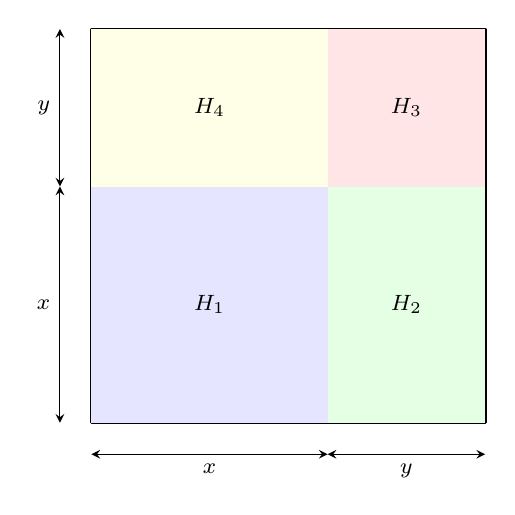
\begin{tikzpicture}[scale=1,line join = round, line cap = round,>=stealth,font=\footnotesize]
				
				% Kích thước
				\def\x{3} % x
				\def\y{2} % y
				
				% Hình vuông lớn
				\draw[line width=1pt] (0,0) rectangle (\x+\y,\x+\y);
				
				% Đường chia dọc và ngang
				\draw (0,\x) -- (\x+\y,\x); % đường ngang
				\draw (\x,0) -- (\x,\x+\y); % đường dọc
				
				% Tô nhẹ các phần
				\fill[blue!10] (0,0) rectangle (\x,\x); % ô vuông x^2
				\fill[green!10] (\x,0) rectangle (\x+\y,\x); % chữ nhật xy
				\fill[yellow!10] (0,\x) rectangle (\x,\x+\y); % chữ nhật xy
				\fill[red!10] (\x,\x) rectangle (\x+\y,\x+\y); % ô vuông y^2
				
				% Ghi nhãn
				\node at (\x/2,\x/2) {$H_1$};
				\node at (\x+\y/2,\x/2) {$H_2$};
				\node at (\x/2,\x+\y/2) {$H_4$};
				\node at (\x+\y/2,\x+\y/2) {$H_3$};
				
				% Ghi độ dài
				\draw[<->] (0,-0.4) -- (\x,-0.4) node[midway,below]{$x$};
				\draw[<->] (\x,-0.4) -- (\x+\y,-0.4) node[midway,below]{$y$};
				
				\draw[<->] (-0.4,0) -- (-0.4,\x) node[midway,left]{$x$};
				\draw[<->] (-0.4,\x) -- (-0.4,\x+\y) node[midway,left]{$y$};
				
		\end{tikzpicture}}
		\loigiai{Hình vuông $H_1$ có diện tích là $S_1=x\cdot x=x^2$.\\
		Hình chữ nhật $H_2$ có diện tích là $S_2=x\cdot y =xy$.\\
		Hình vuông $H_3$ có diện tích là $S_3=y\cdot y=y^2$.\\
		Hình chữ nhật $H_4$ có diện tích là $S_4=x\cdot y=xy$.\\
		Tổng diện tích của $H_1,H_2,H_3,H_4$ là $S=x^2+xy+y^2+xy=x^2+2xy+y^2$.\\
	Ta có $S=x^2+2xy+y^2=(x+y)^2$.}
	\end{bt}
	%Bài 6 
	\begin{bt}%[Dự án EX-9-Đề Cương Toán 8]%[BUINHI]%[8D1V3-1]
	\immini{Một cánh cửa sổ có hình dạng như hình ảnh bên. Ô cửa sổ được cấu tạo bao gồm $1$ hình chữ nhật có chiều rộng là $x$ (dm), chiều dài là $x+2$ (dm) và $2$ hình chữ nhật nhỏ có chiều rộng là $1$ (dm), chiều dài là $x+2$ (dm). Ta cần phải lắp kính của ô cửa sổ này.
	\begin{enumerate}
		\item Viết biểu thức tính tổng diện tích $S$ phần kính cần lắp cho cánh cửa đó theo $x$.
		\item Viết kết quả thành bình phương tổng hoặc hiệu sau đó tính diện tích phần kính của cánh cửa đó với $x=3$ (dm).
		\end{enumerate}
		}{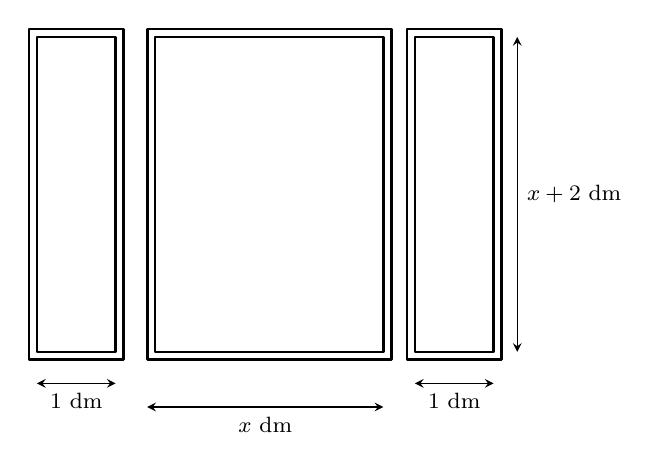
\begin{tikzpicture}[scale=1,line join = round, line cap = round,>=stealth,font=\footnotesize]
			% Thông số
			\def\gap{0.4} % khoảng trống giữa các ô
			
			% Ô nhỏ trái
			\draw[line width=1pt] (0,0) rectangle (1,4);
			\draw[line width=1pt] (-0.1,-0.1) rectangle (1.1,4.1);
			% Ô lớn giữa
			\draw[line width=1pt] (1.1+\gap,0) rectangle (4+\gap,4);
			\draw[line width=1pt] (1+\gap,-0.1) rectangle (4.1+\gap,4.1);
			% Ô nhỏ phải
			\draw[line width=1pt] (4+2*\gap,0) rectangle (5+2*\gap,4);
			\draw[line width=1pt] (3.9+2*\gap,-0.1) rectangle (5.1+2*\gap,4.1);1
%			% Viền đậm bao quanh toàn bộ khung cửa
%			\draw[line width=1pt] (0,0) rectangle (1,4);
%			\draw[line width=1pt] (0,0) rectangle (1,4);
			
			% Ghi kích thước ngang
			\draw[<->] (0,-0.4) -- (1,-0.4) node[midway, below]{$1$ dm};
			\draw[<->] (1+\gap,-0.7) -- (4+\gap,-0.7) node[midway, below]{$x$ dm};
			\draw[<->] (4+2*\gap,-0.4) -- (5+2*\gap,-0.4) node[midway, below]{$1$ dm};
			
			% Ghi chiều cao
			\draw[<->] (5+2*\gap+0.3,0) -- (5+2*\gap+0.3,4) node[midway, right]{$x+2$ dm};

			\end{tikzpicture}} 
		\loigiai{
		\begin{enumerate}
			\item Diện tích phần kính cho cửa sổ hình chữ nhật có kích thước $x \times (x+2)$ là 
				$$S_1=x\cdot (x+2) =x^2+2x \, (\text{dm}^2).$$
			Diện tích phần kính của $2$ ô cửa sổ nhỏ kích thước $1\times (x+2)$ là 
			$$S_2=2 \cdot \left[1 \cdot (x+2) \right]=2x+4 \, (\text{dm}^2).$$
			Tổng diện tích phần kính cần lắp cho  cửa sổ khi đó là 
				$$S=S_1+S_2=(x^2+2x)+(2x+4)=x^2+4x+4 \, (\text{dm}^2).$$
			\item Ta có $S=x^2+4x+4=(x+2)^2$.\\
			Thay $x=3$ vào $S$, ta được $S=(3+2)^2=5^2=25$ (dm$^2$).
		\end{enumerate}}
	\end{bt}
	 %Bài 7 
	 \begin{bt}%[Dự án EX-9-Đề Cương Toán 8]%[BUINHI]%[8D1V3-1]
	 	\immini{Một bạn học sinh thả diều ngoài đồng, cho biết đoạn dây diều từ tay bạn đến diều dài $170$ m. Gọi $x$ là khoảng cách từ bạn học sinh đến vị trí của cánh diều chiếu vuông góc trên mặt đất. Trong điều kiện thời tiết tốt, cánh diều bay căng hết dây và xem như vị trí cánh tay nắm dây diều cao $1{,}5$ m so với mặt đất. 
	 	\begin{enumerate}
	 		\item Lập biểu thức tính độ cao của cánh diều theo $x$;
	 		\item Với $x=80$. Tính độ cao của cánh diều.
	 		\end{enumerate}}
 		{\begin{tikzpicture}[scale=1,>=latex,line join = round, line cap = round,>=stealth,font=\footnotesize]
 				%--- Tọa độ (minh họa, không theo tỉ lệ thực)
 				\coordinate (A) at (0,1.5);   % tay nắm dây (cao 1.5 m)
 				\coordinate (C) at (4,1.5);     % hình chiếu cánh diều trên mặt đất (xa x)
 				\coordinate (B) at (4,5);     % vị trí cánh diều (chiều cao h = 5 trong hình)
 				\coordinate (D) at (4,0);
 				%--- Mặt đất
 				\draw[thick] (-0.5,0) node[left]{Mặt đất} -- (6,0);
 				
 				%--- Tam giác: A-B (dây), B-C (thẳng đứng), C-A (ngang)
 				\draw[thick] (A) -- node[midway,above left] {$170\ \mathrm{m}$} (B); % AB
 				\draw[thick] (B) -- (C); % BC (dọc)
 				\draw[thick] (C) -- (A); % AC (ngang)
 				\draw[thick] (C) -- (D);
 				%--- Đường thẳng vuông góc ở C (kí hiệu góc vuông)
 				\draw ($(D)+(-0.25,0)$) -- ++(0,0.25) -- ++(0.25,0);
 				\draw ($(C)+(-0.25,0)$) -- ++(0,0.25) -- ++(0.25,0);
 				
 				%--- Các điểm và nhãn
 				\fill (A) circle (1.5pt) node[left] {$A$};
 				\fill (C) circle (1.5pt) node[right ] {$C$};
 				\fill (B) circle (1.5pt) node[above right] {$B$ (cánh diều)};
 				\fill (D) circle (1.5pt) node[below right] {$D$};
 				
 				%--- Chú thích kích thước (mũi tên)
 				\draw[<->] ($(A)+(0,-0.05)$) -- ++(0,-1.5) node[midway,right] {$1{,}5\ \mathrm{m}$};
 				\draw[<->] ($(A)+(0,-1.6)$) --($(C)+(0,-1.6)$) node[midway,below] {$x$};
 				\draw[<->] ($(B)+(0.1,0)$) --($(D)+(0.1,0)$) node[midway,right] {$?$};
 		\end{tikzpicture}}
	 		\loigiai{
	 			\begin{enumerate}
	 				\item Áp dụng định lí Pythagore, ta có biểu thức tính độ cao của cánh diều như sau 
	 				$$H=\sqrt{170^2-x^2}+1{,}5.$$
	 			\item Thay $x=80$ vào biểu thức $H$, ta có\\
	 			\begin{eqnarray*}
	 				 H&&=\sqrt{170^2-80^2}+1{,}5\\
	 				 &&=\sqrt{(170-80)\cdot (170+80)}+1{,}5\\
	 				&&=\sqrt{90\cdot 250}+1{,}5=\sqrt{9}\cdot \sqrt{2500}+1{,}5\\
	 				&&=3\cdot 50 + 1{,}5=150+1{,}5=151{,}5\, (m).
	 			\end{eqnarray*}
	 			\end{enumerate}
 			}
	 \end{bt}
	 %Bài 8 
	 \begin{bt}%[Dự án EX-9-Đề Cương Toán 8]%[BUINHI]%[8D1V3-1]
	 Trong một khán phòng dự thính có $36$ chỗ ngồi xếp thành $x$ hàng, tuy nhiên khi đón một đoàn nghiên cứu vào một buổi dự thảo thì phát sinh thêm một số người và cần chuẩn bị thêm ghế ngồi. Phía hậu cần đã thêm $x+2$ ghế vào mỗi hàng do đó nâng tổng số ghế trong khán phòng lên $60$ ghế. Hãy hỏi bên hậu cần đã phải thêm bao nhiêu ghế mỗi hàng?
\loigiai{Tổng số ghế đã thêm vào để đủ chỗ ngồi cho đoàn nghiên cứu là $60-36=24$ (Chỗ ngồi).\\
Theo đề bài, ta có 
\begin{eqnarray*}
	&&x\cdot(x+2)=24\\
    &&x^2+2x-24=0\\
    &&(x^2+2x+1)-25=0\\
    &&(x+1)^2-5^2=0\\
    &&\left[(x+1)-5 \right]\cdot \left[(x+1)+5\right]=0\\
    &&(x-4)(x+6)=0\\
    && x-4=0 \text{ hoặc } x+6=0.\\
    && x=4 \text{ hoặc } x=-6.\\
    && \text{Vì } x\geq 0 \text{ nên } x=4. 
\end{eqnarray*}
Vậy bên hậu cần phải kê thêm $6$ ghế vào mỗi hàng.}
	 \end{bt}
	 %Bài 9
\begin{bt}%[Dự án EX-9-Đề Cương Toán 8]%[BUINHI]%[8D1V3-1]
	Một phòng thí nghiệm đang nghiên cứu một loại kháng thể có tác dụng tăng cường hệ miễn dịch cho cơ thể. Họ tính được công thức tính số lượng kháng thể tăng trưởng trong sau $t$ ngày là $n(t)=8^t$, tỉ lệ vi sinh chết đi trong quá trình tăng trưởng là $8 \colon  3$
	\begin{enumerate}
		\item Viết biểu thức tính số lượng kháng thể có tác dụng được sinh trưởng sau $t$ ngày.
		\item Sau $t$ ngày nuôi trong phòng thí nghiệm, liệu số lượng kháng thể có đủ để phân thành $5$ liều đều nhau hay không?
		\end{enumerate}
	\loigiai{
			\begin{enumerate}
			\item Theo tỷ lệ $8\div 3$ thì số lượng kháng thể chết trong quá trình tăng trưởng là $3^t$.\\
			Số lượng kháng thể có tác dụng sau quá trình tăng trưởng $t$ ngày là $8^t-3^t$.
			\item Ta có \begin{eqnarray*}
				8^t-3^t&&=(8-3)(8^{t-1}+8^{t-2}\cdot 3+8^{t-3}\cdot 3^2+\cdots+8\cdot 3^{t-2}+3^{t-1})\\
				&&=5\cdot (8^{t-1}+8^{t-2}\cdot 3+8^{t-3}\cdot 3^2+\cdots+8\cdot 3^{t-2}+3^{t-1}).
			\end{eqnarray*}
			Như vậy ta có thể thấy lượng kháng thể có tác dụng sau $t$ ngày nuôi vừa đủ để phân thành $5$ liều.
		\end{enumerate}
	}
\end{bt}
	 %Bài 10
	 \begin{bt}%[Dự án EX-9-Đề Cương Toán 8]%[BUINHI]%[8D1V3-1]
	 	Bạn An gửi $10\,000\,000$ VND vào một tài khoản tiết kiệm lãi suất là $x \%\setminus$năm. Lãi suất của bạn An sau một năm sẽ được cộng thêm vào tiền gốc để tiếp tục sinh lãi ở năm tiếp theo. Sau $2$ năm, tổng tiền An nhận được tăng thêm $2\,100\,000$ VND so với số tiền ban đầu. Hỏi lãi suất hàng năm $x$ bằng bao nhiêu?
	 	\loigiai{
	 	Tiền lãi sau năm thứ nhất của bạn An là $10\,000\,000\cdot x\%=10\,000\,000\cdot x\%$ (đồng).\\
	 Tổng tiền vốn và lãi năm đầu tiên sau khi gửi tiết kiệm là
	 $$A_1=10\,000\,000 +10\,000\,000\cdot x\%=10\,000\,000\cdot(1+0{,}01x)\, \text{(đồng)}.$$
	 
	 Tiền lãi của bạn An ở năm thứ hai là $A_1\cdot x\%$ (đồng).\\
	 Tổng tiền vốn lẫn lãi sau hai năm gửi tiết kiệm của An là $$A_2=A_1+A_1\cdot x\%=A_1+A_1\cdot 0{,}01 \cdot x=A_1\cdot (1+0{,}01x)=10\,000\,000\cdot(1+0{,}01x)^2\, \text{(đồng)}.$$
	 	Số tiền tăng thêm so với lúc ban đầu là $$A_2-10\,000\,000=10\,000\,000\cdot \left[(1+0{,}01 x)^2-1 \right]\, \text{(đồng)}.$$
 	Theo đề bài, ta có
	 	\begin{eqnarray*}
 		&&10\,000\,000\cdot \left[(1+0{,}01x)^2-1 \right]=2\,100\,000\\
 		&&(1+0{,}01x)^2-1=0{,}21\\
 		&&(1+0{,}01x)^2-1{,}21=0\\
 		&&(1+0{,}01x)^2-1{,}1^2=0\\
 		&&\left[ (1+0{,}01x)-1{,}1\right]\cdot \left[(1+0{,}01x)+1{,}1\right]=0\\
 		&&(0{,}01x-0{,}1)\cdot(0{,}01x+2{,}1)=0\\
 		&&\text{Vì }x >0\text{ nên }0{,}01x-0{,}1=0\text{ do đó }x=10.
 	\end{eqnarray*}}
	 \end{bt}
	 %Bài 11 
	 \begin{bt}%[Dự án EX-9-Đề Cương Toán 8]%[BUINHI]%[8D1V3-1]
	 	Một khối gỗ có mặt đáy hình vuông cạnh là $a=0{,}5$ m. Trọng lượng của khối gỗ là $500$ N. Sau đó một người thợ đã đóng thêm vào đáy xung quanh khối gỗ các tấm ván hình chữ nhật có kích thước mỗi ván là $x\times\dfrac{(x+2a)}{4}$. Biết rằng công thức tính áp suất của khối gỗ lên bề mặt tiếp xúc với mặt đất là $ P=\dfrac{F}{S}$ (Trong đó $P$ là áp suất (Pa), $F$ lực tạo ra áp suất (N), $S$ là diện tích tiếp xúc (m$^2$)) và trọng lượng các tấm ván đóng thêm là không đáng kể.
	 	\begin{enumerate}
	 		\item Hãy tính diện tích phần đáy của khối gỗ trước và sau khi được đóng thêm các tấm ván ép. Biết $x=0{,}5$.
	 		\item Hãy tính và so sánh áp suất của khối gỗ lên bề mặt trước và sau khi đóng thêm ván gỗ ở ý trên.
	 		\item Viết công thức tính nhanh sự thay đổi diện tích của bề mặt tiếp xúc với độ dài cạnh đáy của khối gỗ. Từ đó đưa ra nhận xét về sự thay đổi của áp suất nếu độ dài cạnh đáy thay đổi theo một tỉ số $k$.
	 		\end{enumerate}
	 		\loigiai{
	 		\begin{enumerate}
	 			\item Diện tích đáy khối gỗ $S_1= a^2=(0{,}5)^2=0{,}25$ m$^2$.\\
	 			Tổng diện tích của $4$ ván gỗ được đóng thêm $S=4 \cdot 0{,}5\dfrac{(0{,}5+2\cdot0{,}5)}{4}=0{,}75$ m$^2$.\\
	 			Diện tích đáy khối gỗ sau khi đóng thêm là $S_2= S_1+S=0{,}25+0{,}75=1$ m$^2$.\\
	 			\item  Áp suất ban đầu của khối gỗ lên mặt đất là $P_1=\dfrac{F}{S_1}=\dfrac{500}{0{,}25}=2\,000$ (Pa).\\
	 			Áp suất của khối gỗ sau khi đóng thêm ván gỗ là $P_2=\dfrac{F}{S_2}=\dfrac{500}{1}=500$ (Pa).\\
	 			Áp suất của khối gỗ sau khi đóng thêm ván gỗ ở đáy giảm $2\,000 \div 500=4$ lần so với ban đầu.
	 			\item Với $a$ là cạnh đáy của khối gỗ và $x$ là độ thay đổi độ dài cạnh đáy thì ta có công thức tính diện tích mặt đáy là $S=a^2+4\cdot x\cdot \dfrac{(x+2a)}{4}=a^2+2ax+x^2=(a+x)^2.$\\
	 			Nếu cạnh đáy của khối gỗ trước và sau thay đổi theo tỉ số $k$ thì áp suất trước và sau sẽ thay đổi theo tỉ số là $\dfrac{1}{k^2}$.
	 		\end{enumerate}}
	 \end{bt}
	 %Bài12 
	 \begin{bt}%[Dự án EX-9-Đề Cương Toán 8]%[BUINHI]%[8D1V3-1]
	 	Có một thực tế rằng, cơ thể một người khi vận động sẽ tiêu tốn nhiều năng lượng hơn trạng thái nghỉ, lượng Oxi cần thiết khi đó cũng tăng lên. Giả sử rằng năng lượng được sinh ra tỉ lệ với bình phương lượng Oxi hấp thu vào cơ thể. Trong trạng thái nghỉ, một người hít vào và hấp thu trung bình $a$ lít O$_2$ mỗi phút sản sinh ra năng lượng $E$ với tỉ lệ là $k=\dfrac{E}{a^2}$. Khi vận động, người đó hấp thu thêm $x$ lít O$_2$ mỗi phút.
	 	\begin{enumerate}
	 		\item  Viết và rút gọn biểu thức tổng quát tính hiệu số năng lượng sinh ra trong $1$ phút giữa hai trạng thái vận động và nghỉ ngơi theo $a,x$ và tỉ số $k$.
	 		\item Với $a=4$ (l/phút), $x=2$ (l/phút) và lấy hệ số tỉ lệ là $k=1$. Tính hiệu số năng lượng sản sinh được. 
	 		\end{enumerate}
	 		\loigiai{
	 			\begin{enumerate}
	 				\item  Năng lượng thu được ở trạng thái nghỉ ngơi là $E_{\text{Nghỉ}}=k\cdot a^2$ (l$^2$/phút$^2$).\\
	 				Năng lượng thu được ở trạng thái vận động là $E_{\text{Vận động}}=k\cdot (a+x)^2$ (l$^2$/phút$^2$).\\
	 				Vậy hiệu số năng lượng giữa hai trạng thái là 
	 				$$E_{\text{Vận động}}-E_{\text{Nghỉ}}=k\cdot \left[ (a+x)^2- a^2\right]=k \cdot \left[ (a+x)- a\right]\cdot \left[ (a+x)+a\right]=kx(2a+x)\, (\text{l}^2/\text{phút}^2).$$
	 				\item Với $a=4$ (l/phút), $x=2$ (l/phút) và hệ số tỉ lệ $k=1$. Hiệu số năng lượng sản sinh được là
	 				$$E_{\text{Vận động}}-E_{\text{Nghỉ}}=kx(2a+x)=1\cdot 2\cdot (2\cdot 4+2)=20\, (\text{l}^2/\text{phút}^2).$$
	 			\end{enumerate}
	 		}
	 	   	 \end{bt}
	 	   	 %Bài 13 
	 	   	 \begin{bt}%[Dự án EX-9-Đề Cương Toán 8]%[BUINHI]%[8D1V3-1]
	 	   	 	Một vật rơi tự do (bỏ qua sức cản của không khí) từ trạng thái nghỉ. Lấy hằng số gia tốc trọng trường $g=10$ m/s$^2$. Quãng đường vật thể rơi được tính theo công thức $s(t)=\dfrac{1}{2}gt^2$ (m).
	 	   	 	\begin{enumerate}
	 	   	 		\item Viết biểu thức tính độ dài quãng đường vật rơi từ thời điểm $t_1$ đến $t_2$ (với $t_1>t_2>0$).
	 	   	 		\item Giả sử vị trí vật rơi cách mặt đất $2\,000$ m. Hỏi từ thời điểm $1$ s đến $19$ s kế tiếp, vật đã rơi được quãng đường là bao nhiêu mét?
	 	   	 		\end{enumerate}
	 	   	 		\loigiai{\begin{enumerate}
	 	   	 				\item Quảng đường vật rơi tại thời điểm $t_1$ $s(t_1)=\dfrac{1}{2}g{t_1}^2$ (m).\\
	 	   	 				Quảng đường vật rơi tại thời điểm $t_2$ $s(t_2)=\dfrac{1}{2}g{t_2}^2$ (m).\\
	 	   	 				Độ dài quãng đường vật rơi từ thời điểm $t_1$ đến $t_2$ là
	 	   	 				$$s(t_2)-s(t_1)=\dfrac{1}{2}g{t_2}^2-\dfrac{1}{2}g{t_1}^2=\dfrac{1}{2}g({t_2}^2-{t_1}^2)\, (\text{m}).$$
	 	   	 				\item Vật rơi từ thời điểm $1$ s đến $19$ s, rơi được quãng đường là 
	 	   	 					$$s(t_2)-s(t_1)=\dfrac{1}{2}\cdot 10\cdot ({19}^2-{1}^2)=\dfrac{1}{2}\cdot 10\cdot (19-1)\cdot(19+1)=\dfrac{1}{2}\cdot 10\cdot 18\cdot 20=1\,800 \,(\text{m}).$$
	 	   	 			\end{enumerate}
	 	   	 		}
	 	   	 \end{bt}